\documentclass[aspectratio=43]{beamer}
\usepackage[utf8]{inputenc}
\usepackage{polski}
% \usepackage[polish]{babel}
\usepackage[T1]{fontenc}
\usepackage{tikz}
\usepackage{tikzducks}
% \usetikzlibrary{decorations.pathmorphing}
\usepackage{multimedia}
\usepackage{graphicx}
\usepackage[justification=centering]{caption}
\usepackage{textcomp}
\usepackage{appendixnumberbeamer}
\usepackage{qrcode}
% \usepackage[natbib, language=polish, sorting=none]{biblatex}
% \addbibresource{lio.bib}
\usepackage{hyperref}
%\usepackage[width=\textwidth]{animate}
%\usepackage{chemformula}
\usepackage{sidecap}
\usepackage{multirow}
\usepackage{rotating}
\usepackage{anyfontsize} % change font size for semposiwko

\usepackage{physics}
\usepackage{array}
\usepackage{booktabs}
\usepackage{transparent}
\usepackage{siunitx}
% \usepackage[rightcaption]{sidecap}
\usepackage{eso-pic}

\usepackage{listings}
\lstset{
basicstyle=\small\ttfamily,
columns=flexible,
breaklines=true
}

% \usepackage{emoji}
\usepackage{subcaption}


\usepackage[natbib, language=polish, sorting=none]{biblatex}
\addbibresource{lio.bib}
\renewcommand*{\bibfont}{\scriptsize}

\usefonttheme[onlymath]{serif}

\usetheme{Szeged}
\usecolortheme{whale}
\setbeamercolor{palette primary}{bg=violet!80!black,fg=white}
\setbeamercolor{palette secondary}{bg=violet!60!black,fg=white}
\setbeamercolor{palette tertiary}{bg=violet!40!black,fg=white}
\setbeamercolor{palette quaternary}{bg=violet!20!black,fg=white}
\setbeamercolor{structure}{fg=violet!60!black}
\setbeamertemplate{caption}{\insertcaption}
% \setbeamertemplate{headline}{
%   \begin{beamercolorbox}[wd=.9\paperwidth]{headline}
%     \vspace{1.5ex}
%     \insertsectionnavigationhorizontal
%     \vspace{1.5ex}
%   \end{beamercolorbox}
% }

\linespread{0.6}

\setbeamertemplate{background}%
{%
    \begin{tikzpicture}[remember picture,overlay]{\node[yshift=1.5cm,xshift=-2cm,opacity=0.1] at (current page.south east)
      {
      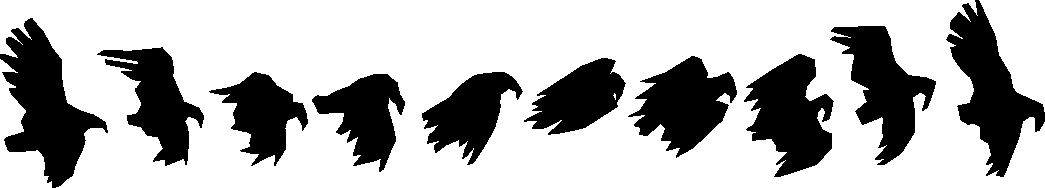
\includegraphics[scale=0.4, angle=20]{ptaki.pdf}
      }
      ;
    \node[yshift=1.0cm,xshift=0.6cm] (logopos) at (current page.south west) {{\begin{tikzpicture}\shuffleducks\duck[signpost=\insertframenumber, \randomhead,scale=.4]\end{tikzpicture}}};
    \pgfmathsetmacro{\progress}{360*(\insertframenumber)/(\inserttotalframenumber)};
    \draw[line width=0.2*3pt] ([xshift=0.55cm] logopos)  arc[radius=0.55cm, start angle=0, end angle=\progress];
    \fill ([shift={(\progress:0.55cm)}] logopos) circle(1pt);

    }
        \end{tikzpicture}
    
}

% \newcommand{\SeMPowisko}{%
% \large S\normalsize%
% \kern-.3em \lower.2ex\hbox{e}%
% \lower.2ex\hbox{\large M\normalsize}%
% \kern-.1em \raise.1ex\hbox{\large P\normalsize}%
% \kern-.3em \lower.2ex\hbox{o}%
% \kern-.2em \raise.2ex\hbox{w}%
% \lower.2ex\hbox{i}%
% s%
% \raise.2ex\hbox{k}%
% \kern-.3em \lower.2ex\hbox{o}%
% }

% \newcommand\Tikz{Ti\emph{k}Z}
% \definecolor{neworange}{RGB}{255,140,0}


\title{Magnetyczny rezonans jądrowy w nanoskali}
\subtitle{kilka wybranych metod}
\author[M. Winiarski]{Mateusz ,,\(\blacksquare\)'' Winiarski}
\institute[Seminarium magisterskie]{biofizyka, FAIS, Uniwersytet Jagielloński}
\date[dzisiaj]{dzisiaj}

\begin{document}

\frame{\titlepage}

\section{Przypomnienie}

\begin{frame}{Przypomnienie}{}

% \begin{itemize}
%     \item 
%     \item 
%     \item 
% \end{itemize}

    \begin{figure}
        \centering
        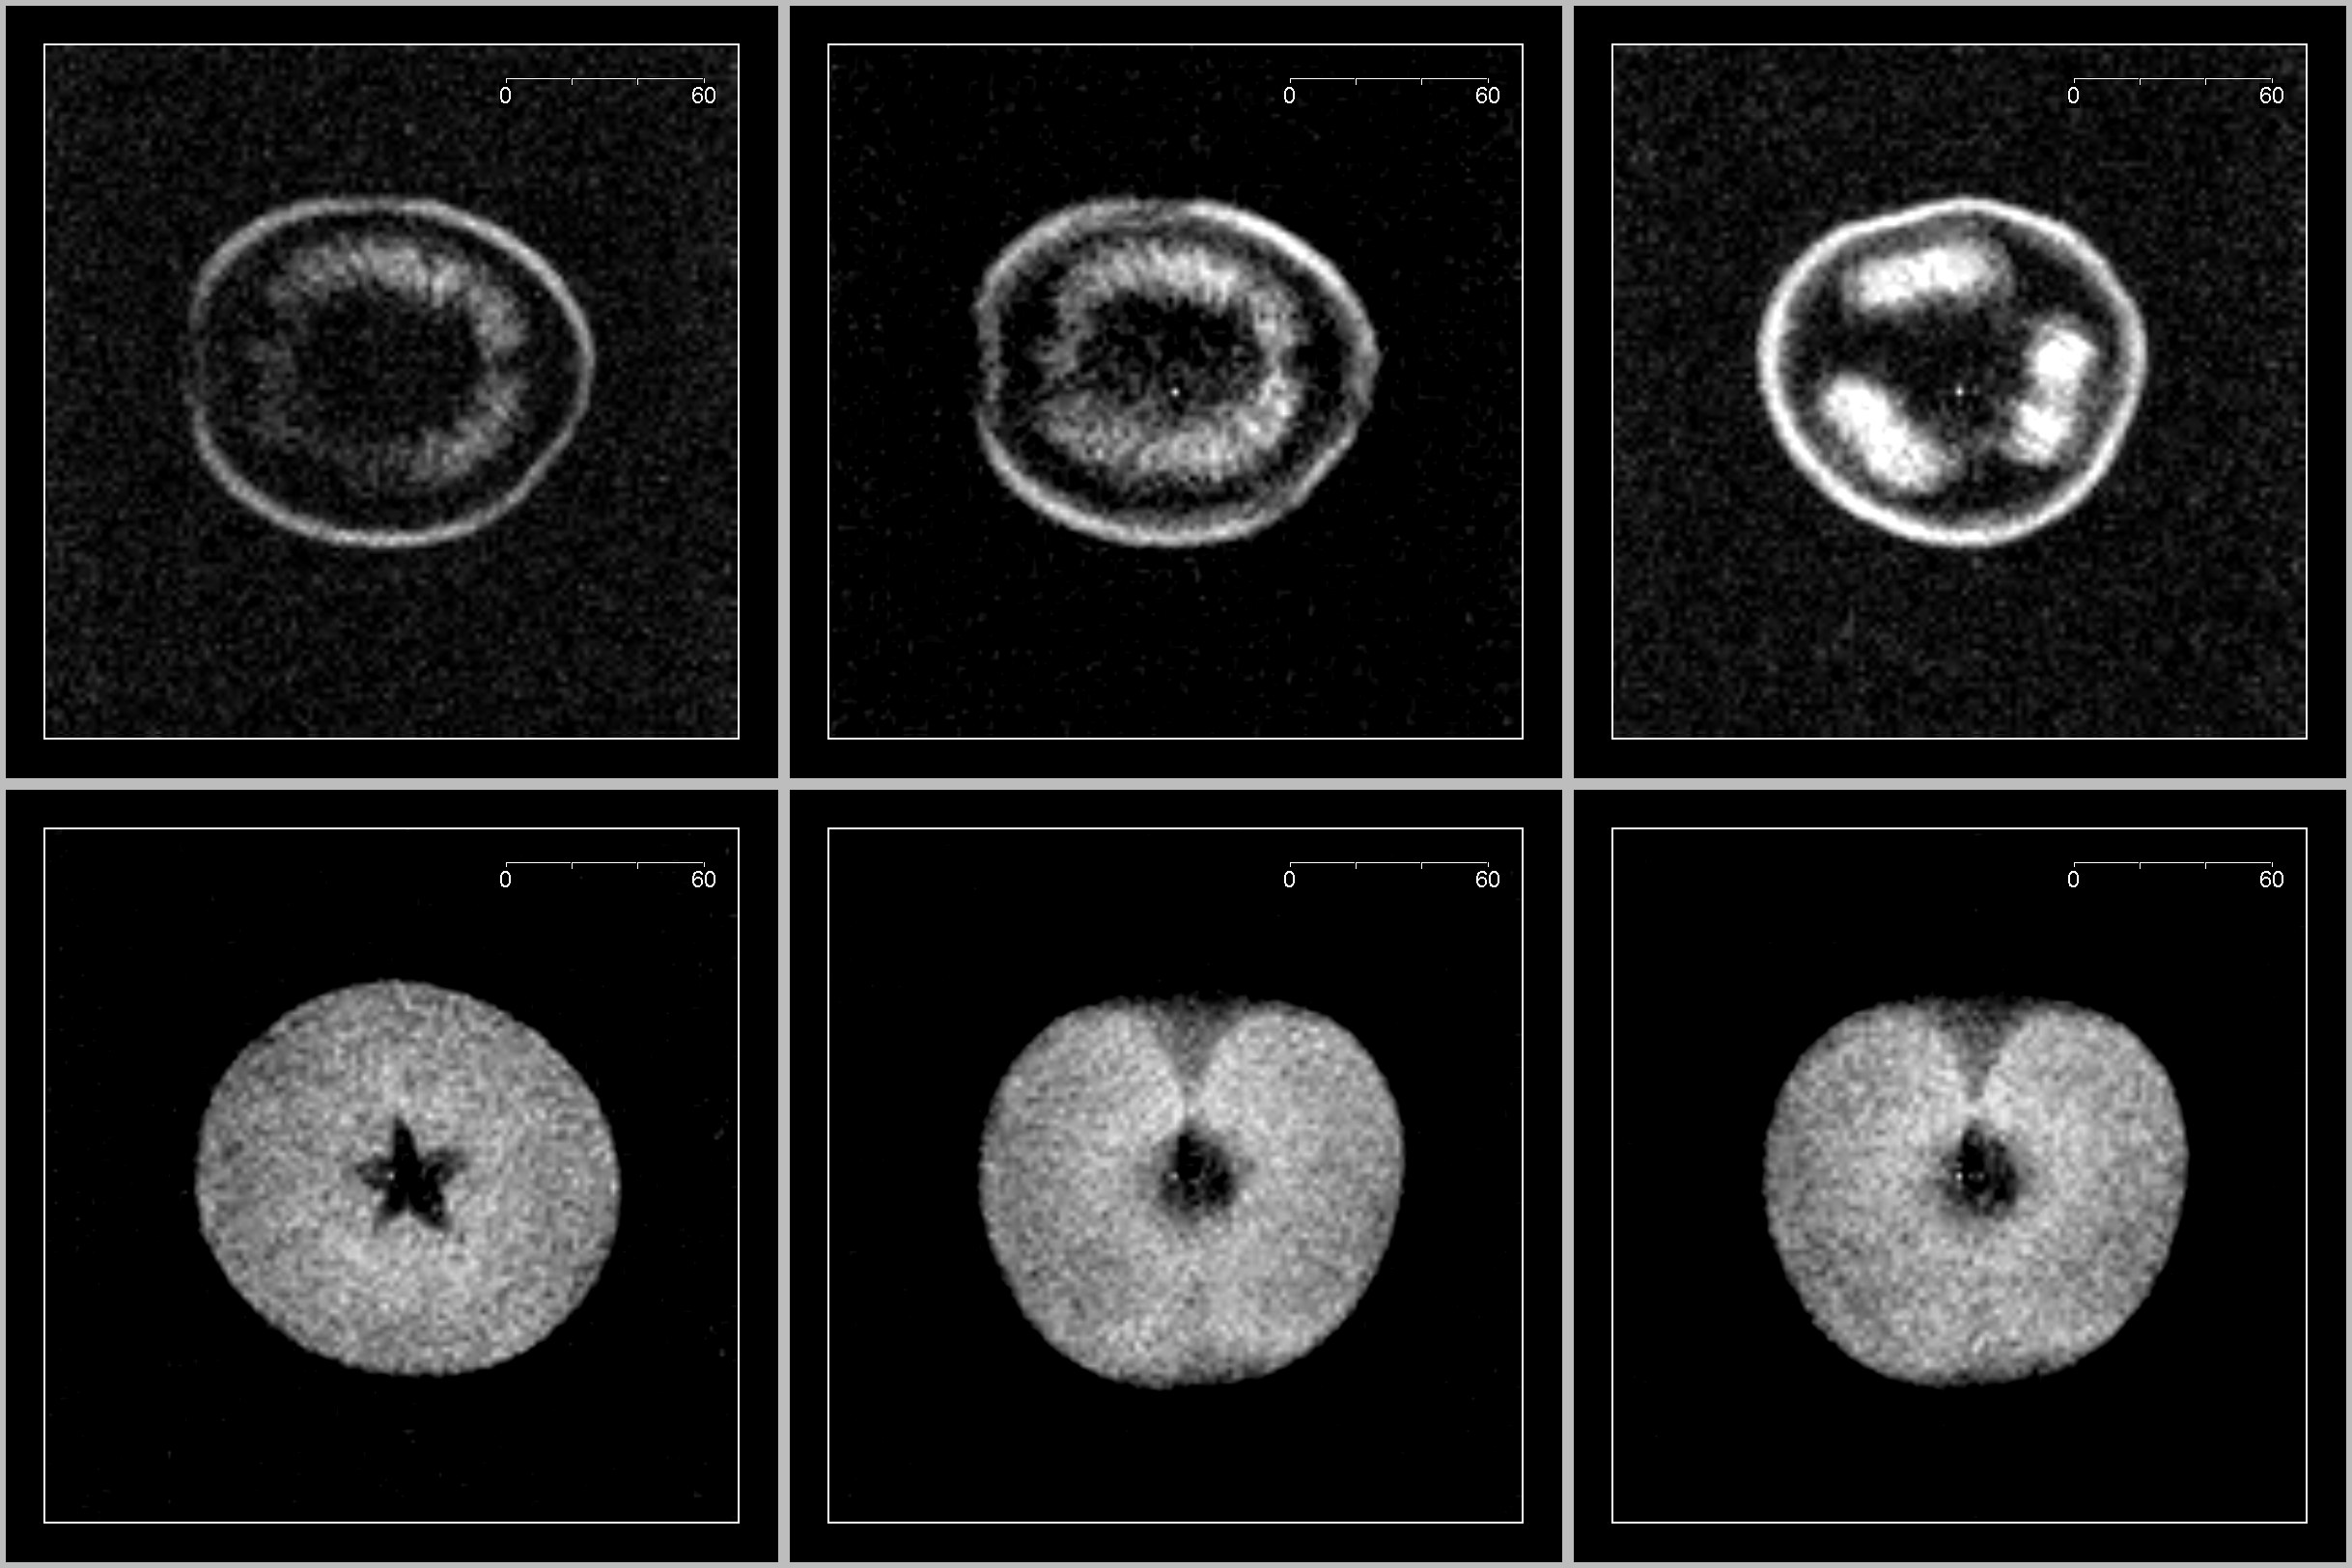
\includegraphics[width=0.6\linewidth]{marakuja_japko.png}
        % \caption{Enter Caption}
        % \label{fig:enter-label}
    \end{figure}
\end{frame}

\begin{frame}{Spis treści}{}
% \small
    \begin{itemize}
        \item \fullcite{Degen_Poggio_Mamin_Rettner_Rugar_2009}
        % \textcolor{fg!50}{
        % \transparent{0.4}
        \item \fullcite{Hammel_2009}
        \item \fullcite{DeVience_Pham_Lovchinsky_Sushkov_Bar-Gill_Belthangady_Casola_Corbett_Zhang_Lukin_etal._2015}
        % }
    \end{itemize}
\end{frame}

\section{MRFM}
\begin{frame}{Spis treści}{}
% \small
    \begin{itemize}
        \item \fullcite{Degen_Poggio_Mamin_Rettner_Rugar_2009}
        % \textcolor{fg!50}{
        \transparent{0.4}
        \item \fullcite{Hammel_2009}
        \item \fullcite{DeVience_Pham_Lovchinsky_Sushkov_Bar-Gill_Belthangady_Casola_Corbett_Zhang_Lukin_etal._2015}
        % }
    \end{itemize}
\end{frame}

\begin{frame}{Metoda działania}
    \begin{columns}
        \column{0.45\textwidth}
        \begin{figure}[0.5]
            \centering
            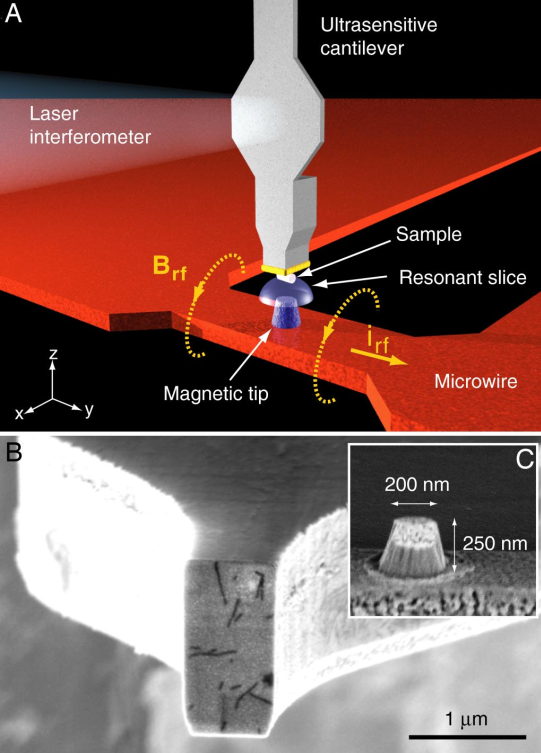
\includegraphics[width=1\linewidth]{mrfm.png}
        \end{figure}
        \column{0.6\textwidth}
        {\scriptsize Konfiguracja aparatury MRFM. 
        \begin{enumerate}[(a)]
        \item Cząstki wirusa mozaiki tytoniowej (TMV), przymocowane do końca ultraczułego krzemowego wspornika, są umieszczone w pobliżu magnetycznej końcówki. Prąd RF \(i_{rf}\) przepływający przez miedziany mikrodrut generuje zmienne pole magnetyczne \(B_{rf}\), które indukuje rezonans magnetyczny w spinach protonowych \({}^1\)H. "Plaster rezonansowy" reprezentuje te punkty w przestrzeni, gdzie pole z magnetycznej końcówki spełnia warunek rezonansu magnetycznego. Trójwymiarowe skanowanie końcówki względem wspornika, a następnie rekonstrukcja obrazu, służą do generowania trójwymiarowego obrazu gęstości spinów w próbce wirusa.
        \item Obraz z mikroskopu elektronowego (SEM) końca wspornika. Poszczególne cząstki wirusa mozaiki tytoniowej są widoczne jako długie, ciemne pręciki na platformie próbki o wymiarach \(0.8-\si{\micro\meter} \times 1.3-\si{\micro\meter}\).
        \item Detale magnetycznej końcówki.
        \end{enumerate}
%         (A)~Tobacco mosaic virus particles,
% attached to the end of an ultrasensitive silicon cantilever, are positioned close
% to a magnetic tip. A rf current \(i_{rf}\) passing through a copper microwire generates an alternating magnetic field \(B_{rf}\) that induces magnetic resonance in the
% 1H spins of the virus particles. The resonant slice represents those points in
% space where the field from the magnetic tip (plus an external field) matches
% the condition for magnetic resonance. Three-dimensional scanning of the tip
% with respect to the cantilever, followed by image reconstruction is used to
% generate a 3D image of the spin density in the virus sample. (B)~Scanning
% electron micrograph of the end of the cantilever. Individual tobacco mosaic
% virus particles are visible as long, dark rods on the \(0.8-\si{\micro\meter} \times 1.3-\si{\micro\meter}\)-sized
% sample platform. (C)~Detail of the magnetic tip.}
}
    \end{columns}
\end{frame}

\begin{frame}{Wyniki obrazowania: wirus TMV}{}
\begin{columns}
\column{0.7\textwidth}
\begin{figure}
    \centering
    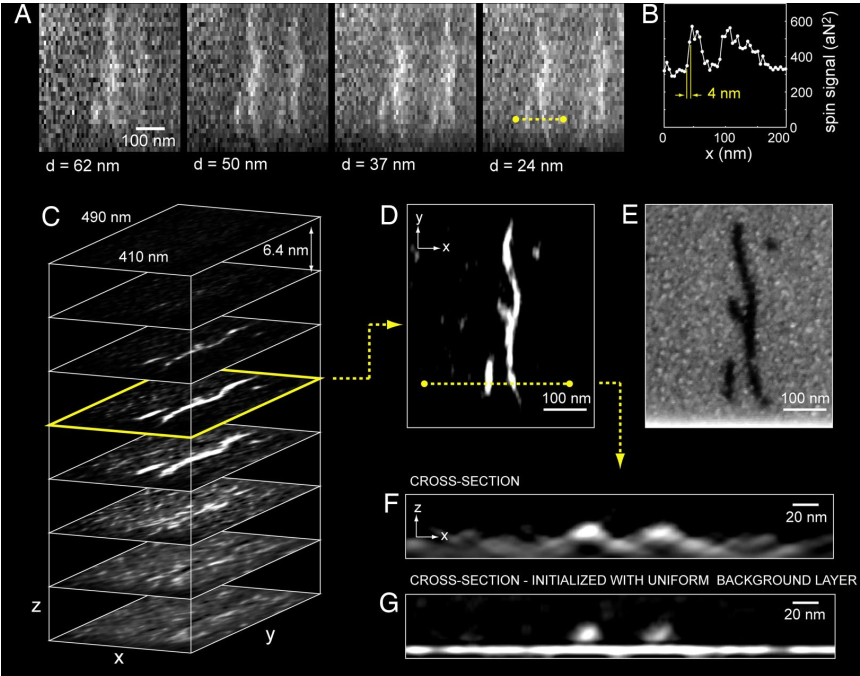
\includegraphics[width=1.1\linewidth]{mr2.png}
    % \caption{Enter Caption}
    % \label{fig:enter-label}
\end{figure}
\column{0.35\textwidth}
{}\hspace{-5cm}
{\scriptsize
\begin{enumerate}[(a)]
    \item Surowe zdjęcia dla różnych odległości końcówka -- próbka.
    \item Skan liniowy na przerywanej linii z (a).
    \item Zrekonstruowana gęstość spinów w 3D.
    \item Horyzontalny przekrój z (c).
    \item SEM tego samego obszaru.
    \item Przekrój przerywanej linii z (d).
    \item Rekonstrukcja obrazu z (f).
\end{enumerate}
}
    \end{columns}
\end{frame}

\section{Azot-wakancja}
\begin{frame}{Spis treści}{}
% \small
    \begin{itemize}
        \transparent{0.4}
        \item \fullcite{Degen_Poggio_Mamin_Rettner_Rugar_2009}
        % \textcolor{fg!50}{
        \transparent{1}
        \item \fullcite{Hammel_2009}
        \transparent{0.4}
        \item \fullcite{DeVience_Pham_Lovchinsky_Sushkov_Bar-Gill_Belthangady_Casola_Corbett_Zhang_Lukin_etal._2015}
        % }
    \end{itemize}
\end{frame}

\begin{frame}{Centra azot-wakancja (NV)}{}
    \begin{figure}
        \centering
        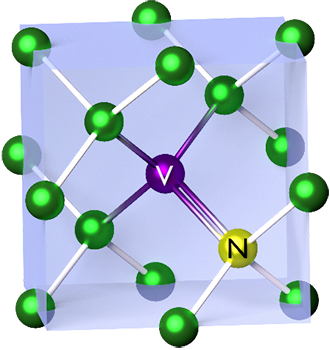
\includegraphics[width=0.4\linewidth]{nv0.png}
        \caption{Uproszczony schemat struktury atomowej centrum azot-wakancja}
        % \label{fig:enter-label}
    \end{figure}
\end{frame}

\begin{frame}{Mechanizm detekcji I}{}
    \begin{figure}
        \centering
        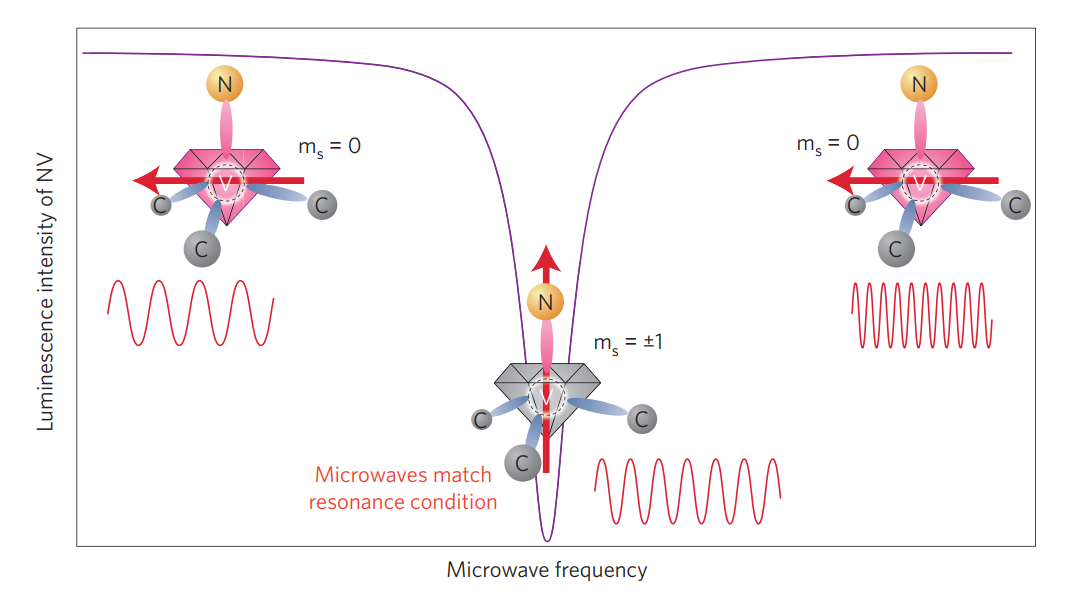
\includegraphics[width=0.8\linewidth]{nv1.png}
        
%         \footnotesize Optical detection of the magnetic resonance of a NV diamond centre. The spin state of
% an electron (red arrow) associated with an NV centre, and hence its manipulation using magnetic
% resonance, is detected via its influence on the optical luminescence. The luminescence is bright when
% the spin state is in the quantum mechanical state \(m_s = 0\) and darker when in the other two states:
% \(m_s = +1\) or \(m_s = –1\). Magnetic resonance induces transitions between the \(m_s = 0\) and \(m_s = \pm1\) levels when
% microwaves (indicated by the sine waves) are applied. The laser light that causes luminescence also
% initializes spin(s) to the \(m_s = 0\) state. Hence, when microwaves in resonance with the spin oscillations
% shift the spin to the \(m_s = \pm1\) state the luminescence changes and this can be picked up by a highly
% sensitive detector. Resonance of a single NV centre can be measured in ambient conditions.
% \caption{
{\scriptsize Optyczna detekcja rezonansu magnetycznego centrum NV w diamencie. Stan spinowy elektronu w centrum NV (oznaczony jako \(m_s = 0\), \(m_s = +1\) lub \(m_s = -1\)) wpływa na luminescencję, która jest większa dla stanu \(m_s = 0\) i mniejsza dla stanów \(m_s = \pm 1\). Mikrofale indukują przejścia między tymi stanami, a zmiany w luminescencji są rejestrowane przez czuły detektor, co pozwala na pomiar rezonansu magnetycznego pojedynczego centrum NV w warunkach otoczenia.}
% }
        % \label{fig:enter-label}
    \end{figure}
\end{frame}

\begin{frame}{Mechanizm detekcji II}{}
    \begin{figure}
        \centering
        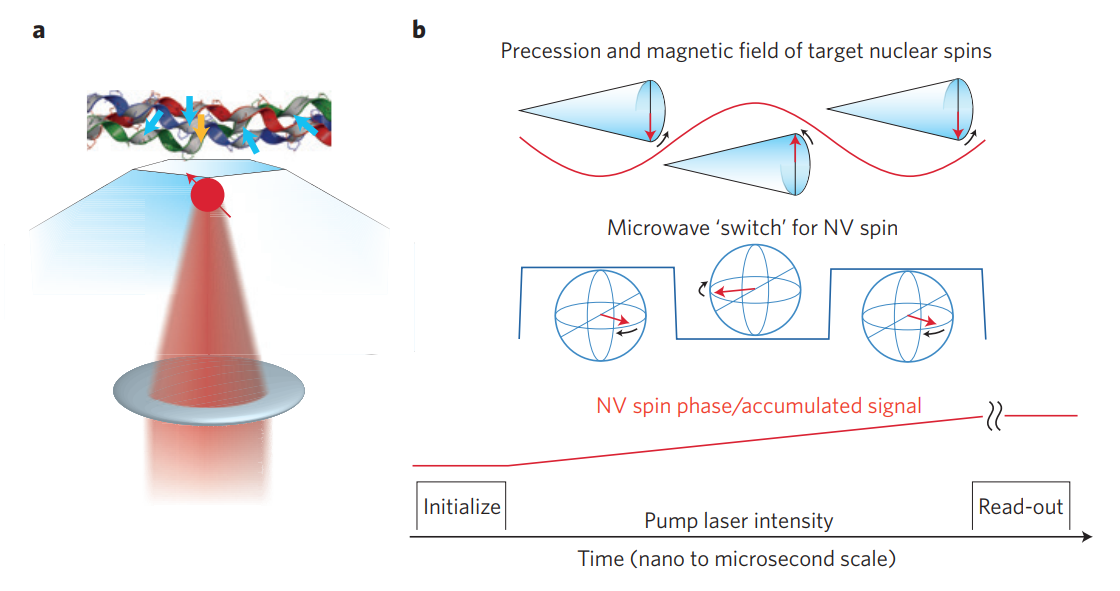
\includegraphics[width=0.75\linewidth]{nv2.png}
        
        % {\scriptsize Pomiar pola magnetycznego jądra atomowego oscylującego z częstotliwością rezonansową. Jądra (np. w biomolekułach) znajdują się w pobliżu centrum NV w diamencie, a ich oscylacje generują oscylujące pole magnetyczne, które jest wykrywane przez spin elektronu w centrum NV. Mikrofalowe impulsy są używane do manipulacji spinem NV, co pozwala na detekcję zmian w polu magnetycznym i pomiar rezonansu jądrowego.}
        {\scriptsize (a) Biomolekuła znajdująca się blisko centrum NV w diamencie. Centrum NV działa jako detektor, a jego luminescencja jest monitorowana podczas manipulacji mikrofalami, co umożliwia selektywną detekcję pól magnetycznych generowanych przez jądra.
        
        (b) Jądra atomowe precesują w zewnętrznym polu magnetycznym, generując oscylujące pole magnetyczne. Impulsy mikrofalowe są używane do przełączania spinu elektronu w centrum NV, co pozwala na detekcję zmian w polu magnetycznym. Jeśli częstotliwość precesji jąder jest dokładnie połową częstotliwości przełączania spinu NV, spin NV akumuluje fazę, co prowadzi do zmiany w luminescencji, która jest mierzona.}
    \end{figure}
\end{frame}

\section{Azot-wakancja 2: Tokyo Drift}
\begin{frame}{Spis treści}{}

\AddToShipoutPicture*{
    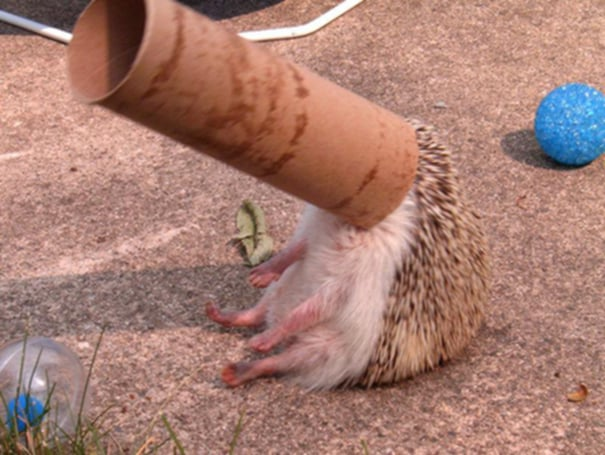
\includegraphics{jez.png}
}

% \small
    \begin{itemize}
        \transparent{0.4}
        \item \fullcite{Degen_Poggio_Mamin_Rettner_Rugar_2009}
        % \textcolor{fg!50}{
        \item \fullcite{Hammel_2009}
        \transparent{1}
        \item \fullcite{DeVience_Pham_Lovchinsky_Sushkov_Bar-Gill_Belthangady_Casola_Corbett_Zhang_Lukin_etal._2015}
        % }
    \end{itemize}
\end{frame}

\begin{frame}{Mechanizm detekcji mikroskopowej}{}

\begin{figure}
    \centering
    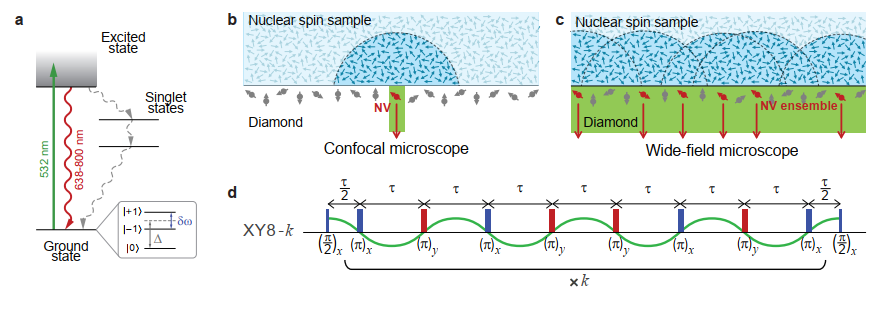
\includegraphics[width=0.95\linewidth]{nw1.png}
    % \caption{Enter Caption}
    % \label{fig:enter-label}

    {\scriptsize
    \begin{enumerate}[(a)]
        \item Diagram poziomów energetycznych centrum NV.
        \item Metoda działania z użyciem mikroskopii konfokalnej.
        \item Metoda działania z użyciem mikroskopii szerokiego pola.
        \item Precesja Larmora produkuje zmienne pole magnetyczne, wykrywane przez sekwencję pulsów XY8-\(k\).
    \end{enumerate}
    }
\end{figure}
    
\end{frame}

\begin{frame}{Wyniki I: próbki fluorowane}
    \begin{figure}
        \centering
        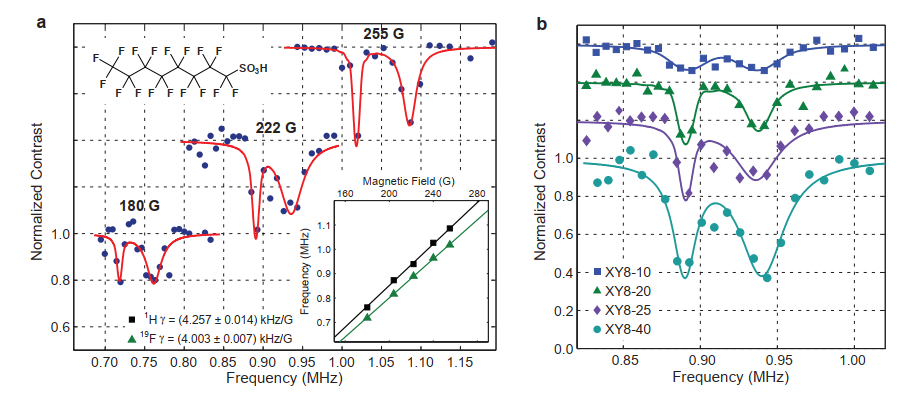
\includegraphics[width=1\linewidth]{nw2.png}
        % \caption{Enter Caption}
        % \label{fig:enter-label}
    {\scriptsize
    Wielojądrowa spektroskopia NMR w skali nanometrowej z wykorzystaniem pojedynczego płytkiego centrum NV.
    \begin{enumerate}[(a)]
        \item Widma NMR dla jąder \({}^1\)H (wodór) i \({}^{19}\)F (fluor) w próbce fluorowanej (PFOS/POSF) przy różnych polach magnetycznych, zmierzone za pomocą sekwencji impulsów XY8-10.
        \item Seria widm NMR dla próbki fluorowanej, uzyskanych przy rosnącej liczbie powtórzeń \(k\) sekwencji impulsów XY8-\(k\).
    \end{enumerate}
    }
    \end{figure}
\end{frame}

\begin{frame}{Wyniki II: próbki fluorowane}{}
\begin{figure}
    \centering
    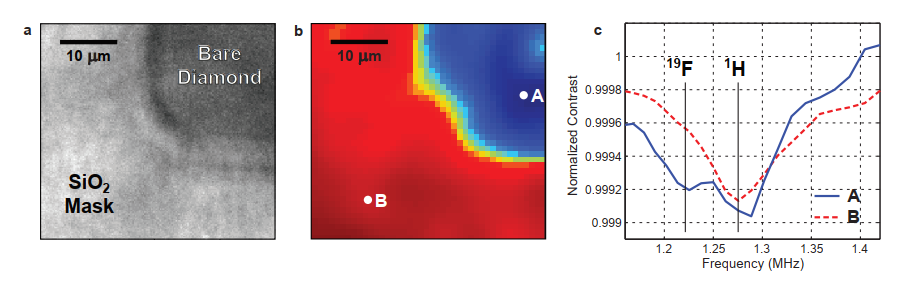
\includegraphics[width=\linewidth]{nw4.png}
    % \caption{Enter Caption}
    % \label{fig:enter-label}
    {\scriptsize
    \begin{enumerate}[(a)]
        \item Diagram poziomów energetycznych centrum NV.
        \item Obraz MRI gęstości spinów \(^{19}\)F: niebieski -- wysoki kontrast, czerwony -- brak sygnału.
        \item Spektrum NV NMR w punktach A i B.
    \end{enumerate}
    }
\end{figure}
    
\end{frame}

%end frame

\section{}

\begin{frame}{}

\begin{figure}

\centering
    \begin{tikzpicture}
      \duck[parrot, body=gray!30!yellow, head=gray!30!yellow, bill=red, torch=gray!70!brown, tshirt=red!40!black, ribbon=gray, bowtie=blue!50!white, crazyhair=black]
      %\addwater{blue!50!cyan}
      \fill[cyan!20!white] (-1.4,1.8) ellipse (1.8 and 0.5);
  \fill[cyan!20!white] (-0.2,1.54) -- (0.2,1.35) -- (0.0,1.6) -- cycle;
	\node at (-1.4,1.8) {dziękuję za uwagę};
    \end{tikzpicture}
    \end{figure}


    
    \begin{figure}
    \centering
    \qrcode[height=0.3\textwidth]{https://github.com/falcotinnunculus/przezrocza/blob/wladca/nm/main.pdf}\\
    {\tiny \url{https://github.com/falcotinnunculus/przezrocza/blob/wladca/nm/main.pdf}}

    \end{figure}
\vspace{-4.15cm}
\transparent{0.5}
    \begin{figure}
        \centering
        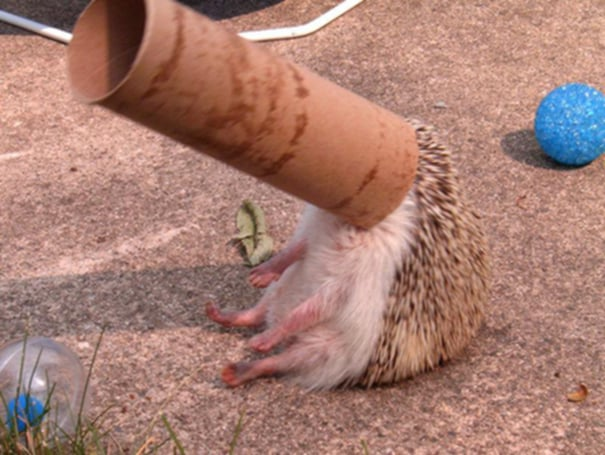
\includegraphics[height=0.3\linewidth]{jez.png}
        % \caption{Caption}
        % \label{fig:enter-label}
    \end{figure}
\end{frame}


\end{document}